\subsection{Proposed workaround}

% What's the plan to fix that crap
As it was identified earlier, a single failure criteria for modeling the output waveform is the main cause of error.
A modification to the characterization method is proposed.

% What is kept in the method, What is modified
The characterization is still performed per-block, still by injecting variable width and variable amplitude rectangular pulses on an input.
However, the failure criteria on the output is now eliminated.
Instead, two values are recorded rather than one.
First, the maximum amplitude value on the output is measured.
Second, the width of the disturbance is also sampled.
It is measured at a fixed percentage of the maximum amplitude.

% What value and why ?
In our current study case, a value of 90\% was employed.
It provides some noise-margin against voltage fluctuations near maximum amplitude during the pulse.
The concept is illustrated in Fig. \ref{fig:impact-single-failure-criteria}.
Basically, this method can be seen as modelling and simplifying a complex waveform into a rectangular waveform.

\begin{figure}[!h]
  \centering
  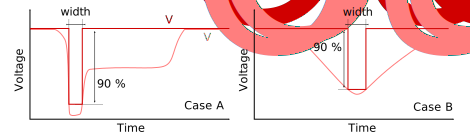
\includegraphics{src/4/figures/better_output_modelling.pdf}
  \caption{Improved output modelling method based on 90\% of maximum disturbance amplitude}
  \label{fig:impact-single-failure-criteria}
\end{figure}

% Result, 2 curves - explain what they are.
Since two parameters are now recorded, two curves are obtained per block rather than one.
The first curve is $out_{amplitude} = f(in_{width}, in_{amplitude})$.
The second curve is $out_{width} = f(in_{width}, in_{amplitude})$.

% What is the improvement
These two curves constitute the model of the block.
Like done previously, models are chained together to deduce the robustness of a complete function.
Fig. \ref{fig:full-method-v2} illustrates the entire characterization and chaining process using these two curves per model.

\begin{figure}[!hp]
  \centering
  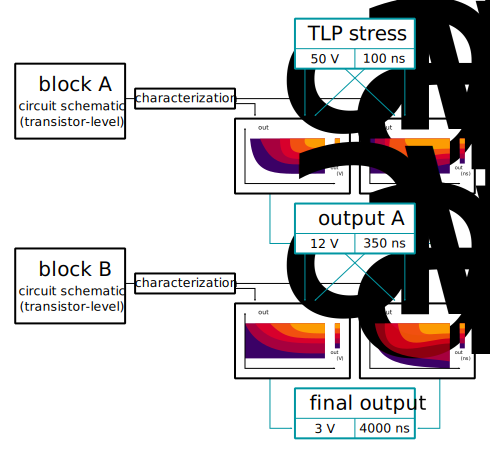
\includegraphics{src/4/figures/full_method_overview_v2.pdf}
  \caption{Overview of improved bottom-up method - example with two blocks}
  \label{fig:full-method-v2}
\end{figure}

% Explain the figure
After each block is characterized, a \gls{tlp} stress is applied to the first model.
In this example, the pulse has an amplitude of 50V ($in_{amplitude}$) and a width of 100ns ($in_{width}$).
The first curve indicates the output is disturbed with a maximum amplitude of 12V ($out_{amplitude}$).
The second curve indicates the output is disturbed during 350ns ($out_{width}$).
These two values can now be applied to the model of block B with the same process.
Finally, it is found that the output is disturbed at a maximum amplitude of 3V during 4000ns.

\subsection{Application to the testchip}

% Apply to the teschip
The new method is applied to the same three blocks of the testchip for checking its validity.
The pre-regulator is characterized first (Figs \ref{fig:pre-reg-cz-v2-amp} and \ref{fig:pre-reg-cz-v2-width}).

\begin{figure}[!h]
  \centering
  \includegraphics[width=0.95\textwidth]{src/4/figures/vpre_cz_V2_amplitude.png}
  \caption{Pre-regulator characterization - $min(V_{out}) = f(V_{in}, W_{in})$}
  \label{fig:pre-reg-cz-v2-amp}
\end{figure}

\begin{figure}[!hp]
  \centering
  \includegraphics[width=0.95\textwidth]{src/4/figures/vpre_cz_V2_width.png}
  \caption{Pre-regulator characterization - $W_{out} = f(V_{in}, W_{in})$}
  \label{fig:pre-reg-cz-v2-width}
\end{figure}

% Detail graph - pre-reg amplitude
Fig. \ref{fig:pre-reg-cz-v2-amp} plots a gradient representing the minimal amplitude of the output signal,
in function on the input stress characteristics (amplitude and width).
The characterized block is the pre-regulator.
It plots the \textbf{minimal} amplitude and not the \textbf{maximal} amplitude because the input stress is negative.
Therefore, a smaller value on the output means a larger disturbance.

% Analysis
It can be noticed that the output voltage is mostly dependent on the input voltage, and not on the input pulse width.

% Detail graph - pre-reg width
Fig. \ref{fig:pre-reg-cz-v2-width} is the second curve obtained by characterizing the pre-regulator.
It plots a gradient representing the disturbance width of the output, in function on the input voltage.
The width of the disturbance is calculed by at 90\% of the minimum output amplitude.

% Analysis
This output width characteristic is quite different from the previous output voltage characteristic.
Here, the output width depends on both the input amplitude and input width.
For input voltages mostly above 2V, the output width does not depend on the input width.
It is exclusively tied to the input voltage.
Then, below 2V, this behavior becomes reversed. The output width is directly dependent on the input width,
no matter the input voltage.
%TODO: Try to explain why

% Summarize
Both Figs. \ref{fig:pre-reg-cz-v2-amp} and \ref{fig:pre-reg-cz-v2-width} constitute the pre-regulator model.

\begin{figure}[!htb]
  \centering
  \includegraphics[width=0.95\textwidth]{src/4/figures/bandgap_cz_V2_amplitude.png}
  \caption{Bandgap characterization - $min(V_{out}) = f(V_{in}, W_{in})$}
  \label{fig:bandgap-cz-v2-amp}
\end{figure}

\begin{figure}[!htb]
  \centering
  \includegraphics[width=0.95\textwidth]{src/4/figures/bandgap_cz_V2_width.png}
  \caption{Bandgap characterization - $W_{out} = f(V_{in}, W_{in})$}
  \label{fig:bandgap-cz-v2-width}
\end{figure}

% Analyse bandgap cz
The bandgap is also characterized with the exact same approach.
The output amplitude curve in Fig. \ref{fig:bandgap-cz-v2-amp} has mostly an input-amplitude dependency, except for large voltage disturbances.
The output width curve in Fig. \ref{fig:bandgap-cz-v2-width} has a clear input voltage and width dependency.
This means the output is disturbed because of an energy level, not just a signal level.

%TODO: Inverse colorscale - small amplitude means more disturbed
\begin{figure}[!htb]
  \centering
  \includegraphics[width=0.95\textwidth]{src/4/figures/regulator_cz_V2_amplitude.png}
  \caption{Regulator characterization - $min(V_{out}) = f(V_{in}, W_{in})$}
  \label{fig:reg-cz-v2-amp}
\end{figure}

%TODO: Fix the colorscale
\begin{figure}[!htb]
  \centering
  \includegraphics[width=0.95\textwidth]{src/4/figures/regulator_cz_V2_width.png}
  \caption{Regulator characterization - $W_{out} = f(V_{in}, W_{in})$}
  \label{fig:reg-cz-v2-width}
\end{figure}

% Analyse regulator cz
Finally, the regulator is also characterized.
The output amplitude curve in Fig. \ref{fig:reg-cz-v2-amp} has a clear input voltage and width dependency.
Therefore, the output voltage is disturbed because of an excedent energy on the input.
A large-amplitude short pulse and a small-amplitude long pulse should the disturb the output almost identically.

The output width curve in Fig. \ref{fig:reg-cz-v2-amp} is the most complex of all to interpretate.
Both voltage and width impact the output.
Beyond an input width of 7500ns, the output is suddenly heavily disturbed.
Just below 7300ns, the curve value is XXXX ns.
At 7500ns, the output width is now XXXXns.
This specific area of the curve looks like a clear soft-failure, where the system suddenly goes into reset or safe-mode, and a long procedure to restart it happens.

% Conclusion ?
%TODO
Input voltage output voltage no direct relation
width also plays a role

% Apply a TLP to the models
These models are now used to predict a failure on the final block output when injecting a \gls{tlp} stress on the first input.
A program was written to automate this process.
Before comparing the models

The results obtained with the models are compared to a full transistor-level simulation given in Fig. \ref{fig:reference_simu_v2}.

REF Simulation

A first comparison is given in Table. \ref{tab:model-v2-vs-sim} for a (100ns, -30V) input stress.

\begin{table}[!h]
\centering
\begin{tabular}{@{}lllllllll@{}}
           & \multicolumn{2}{l}{vclamp9}          & \multicolumn{2}{l}{vref1p0}          & \multicolumn{2}{l}{v2p5}               \\
\toprule
models     & 92 ns  & \textcolor{red!90}{-4.51 V} & 85 ns & \textcolor{red!90}{-3.55 V}  & \textcolor{red!90}{185 ns} & \textcolor{blue!90}{2.41 V} \\
simulation & 101 ns & -2.19 V                     & 87 ns & -0.91 V                      & 337 ns      & 2.26 V
\end{tabular}
\caption{Model application for (100ns, -50V) input stress}
\label{tab:model-v2-vs-sim}
\end{table}

% What correlates in the first table
This new characterization method seems to be a major improvement over the first one (described previously in \ref{sec:block-failure-cz}).
The pre-regulator's output is estimated to be disturbed during 92 ns, with only 9 ns of difference with the reference simulation.
Similarly, the bandgap's output is estimated to be disturbed during 85 ns, with an error of only 2 ns.
For these first two blocks, the models seem to predict correctly the disturbance width.

% What does not correlate
On the other hand, the model does not correlate well with the reference simulation for the regulator's output .
The disturbance's width is estimated at 185 ns, which is almost half the reference value of 337 ns.
The disturbance's amplitude obtained with the models is extremely close to the nominal value.
It would mean that the output should almost not be disturbed.
In practice, the reference simulation shows that the simulation is disturbed and drops at 2.26 V.

% preliminary conclusion
As a preliminary conclusion, the models estimate correctly the disturbance's duration.
The width obtained for the regulator is wrong, but it might be a particular case where the width is not recorded properly.
The models however require improvements for predicting the disturbed amplitude.
The models are tested once again against the reference for different input pulses (tables \ref{tab:model-v2-vs-sim-2} and \ref{tab:model-v2-vs-sim-3}).

\begin{table}[!h]
\centering
\begin{tabular}{@{}lllllllll@{}}
           & \multicolumn{2}{l}{vclamp9}           & \multicolumn{2}{l}{vref1p0} & \multicolumn{2}{l}{v2p5} \\
\toprule
models     & 92 ns  & \textcolor{red!90}{-11.42 V} & 61 ns       & -3.55 V       & \textcolor{red!90}{184 ns} & \textcolor{blue!90}{2.41 V}     \\
simulation & 101 ns & -4.00 V                      & 94 ns       & -2.63 V       & 341 ns                     & 2.25 V
\end{tabular}
\caption{Model application for (100ns, -200V) input stress}
\label{tab:model-v2-vs-sim-2}
\end{table}

\begin{table}[!h]
\centering
\begin{tabular}{@{}lllllllll@{}}
           & \multicolumn{2}{l}{vclamp9}            & \multicolumn{2}{l}{vref1p0} & \multicolumn{2}{l}{v2p5} \\
\toprule
models     & 1000 ns & \textcolor{red!90}{-11.48 V} & 894 ns       & -3.64 V      & \textcolor{red!90}{293 ns}  & 2.27 V     \\
simulation & 1000 ns & -4.87 V                      & 613 ns       & -3.43 V      & 698 ns                      & 2.06 V
\end{tabular}
\caption{Model application for (1us, -200V) input stress}
\label{tab:model-v2-vs-sim-3}
\end{table}

% What is correlating, what is not
The width is well predicted for the pre-regulator (\textit{vclamp9}) and bandgap (\textit{vref1p0}) models.
There is an issue however with the regulator's model, that underestimates the simulated duration on \textit{v2p5}.
Also, amplitude are not estimated correctly in general.

% Look at v2p5 for explaining differences
Overall, the regulator model is the less accurate one.
To understand those differences, the reference simulation waveform is compared to the model's waveform.
The reference simulation is run with a (100 ns, -200V) pulse injected on \textit{vbatt}.
It should result in a (94 ns, -2.63 V) disturbance on the input of the regulator. NOPE!
The model's simulation is run by a injecting the same (94 ns, -2.63 V) pulse on the regulator's input.
This pair of values is obtained from table \ref{tab:model-v2-vs-sim-2}.

%TODO: Show a characterization simu first block wvf versus full simu first block output

%TODO: Interpret simulation comparison

Input waveform is not modeled properly. Much wider than expected.
Pulse width seems to have the largest impact on the regulator than pulse amplitude

Final sources of error : 90\% limit, that could benefit from a 10\% limit, and difference between the actual study case and the characterization schematics.

\subsection{Final limitations and conclusion}

% Opening on how to improve the modeling
Characterization could be improved by using multiple thresholds and obtain width at those multiple thresholds.
A more accurate model of the output could be derived.
Ideally, the integral of the output waveform and the model waveform should be compared, and if a too large difference appears, more thresholds should be used.

%TODO: Figure

Ultimately, the goal is to build a simpler representation of the output waveform of a block, composed of square shapes.
The main advantage of those shape is that they are understood by the block models.
It could be seen as a mathematical transformation of a time-domain waveform into a square-domain waveform.

% What are the final limits of this method
How to handle real circuit topology (interconnect mesh) versus the linear one used in the characterization.
Talk about 1 pin to many pin that is ok, but many pin to 1 is not covered at all by this method
